\documentclass{beamer}
%
% Choose how your presentation looks.
%
% For more themes, color themes and font themes, see:
% http://deic.uab.es/~iblanes/beamer_gallery/index_by_theme.html
%
\mode<presentation>
{
  \usetheme{default}      % or try Darmstadt, Madrid, Warsaw, ...
  \usecolortheme{default} % or try albatross, beaver, crane, ...
  \usefonttheme{default}  % or try serif, structurebold, ...
  \setbeamertemplate{navigation symbols}{}
  \setbeamertemplate{caption}[numbered]
} 

\usepackage[english]{babel}
\usepackage[utf8x]{inputenc}
\usepackage{amsmath,amsthm,amssymb,amsfonts}
\newtheorem*{dfn}{Definition}
\newtheorem{thm}{Theorem}[subsection]
 \renewcommand{\thethm}{\arabic{thm}}
%\newtheorem{lemma}{Lemma}
\title[Introduction]{Statistics Learning Theory:Logistic Regression}
\author{}
\institute{}
\date{2019.02.23}

\begin{document}

\begin{frame}
  \titlepage
\end{frame}

% Uncomment these lines for an automatically generated outline.
%\begin{frame}{Outline}
%  \tableofcontents
%\end{frame}

\section{Logistic Regression}
\begin{frame}{Logistic Regression:Sigmoid Function}
	In this week slide, we will introduce the implementation of Logistic regression and related property. \\
	To understand the method of logistic regression, we first introduce the sigmoid function. That is, the function $\sigma_{sig}:R \rightarrow [0,1]$ over the class of linear functions $L_d$ such that
	\[\sigma_{sig}(z) = \frac{1}{1+exp(-z)}\]
	The hypothesis class becomes
\[\mathcal{H} = \sigma_{sig} \circ L_d = \{x \rightarrow \sigma_{sig}(\langle w,x \rangle)): w \in R^d\}\]
\end{frame}
\begin{frame}{Logistic Regression:Loss function}
	Given the classifier $h_{w}(x)$, we should define how bad it is to predict some $h_w(x) \in [0,1]$ given that the true label is $y \in \{1,-1\}$ \\
	Therefore, we would like that $h_w(x)$ would be large if $y=1$ and that $1-h_w(x)$ would be large if $y=-1$. Since
	\[1 - h_w(x) = \frac{1}{1+exp(\langle w,x \rangle)}\]
	Therefore, any resonable loss function would increase monotonically with $\frac{1}{1+exp( y \langle w,x \rangle)}$
\end{frame}
\begin{frame}{Logistic Regression:Loss function}
	We can choose the log function, that is the loss function
	\[l(h_w,(x,y)) = \log (1+exp( -y \langle w,x \rangle)\]
	The ERM problem associated with logistic regression is 
	\[arg\min_{w \in R^d} \frac{1}{m} \sum^m_{i=1} \log(1+exp( -y \langle w,x \rangle)\]
\end{frame}
\begin{frame}{Logistic Regression: Remark}
	\begin{enumerate}
		\item logistic loss function is convex function, the optimization can be solved efficienyly
		\item The ERM problem associated with logistic regress is identical to the problem of finding a maximimum Likelihood Estimator.
	\end{enumerate}
\end{frame}
\begin{frame}
	 \begin{block}{Sigmoid function}
		 % Your image included here
		 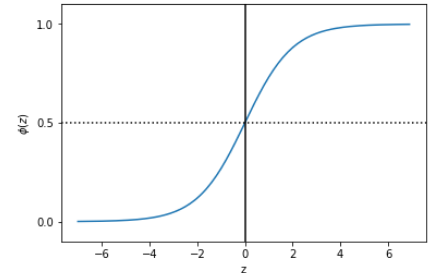
\includegraphics[width=\textwidth]{Sigmoid.png}
	\end{block}
\end{frame}
\end{document}
